\documentclass{acmsiggraph}

\usepackage{parskip}
\usepackage{graphicx}
\usepackage{footmisc}
\usepackage{amsmath}
\usepackage{url}
\onlineid{0}

\title{\Large Plotting the Single-Electron Solution to Schr\"{o}dinger's Equation with OpenCL}

\author{Tim Horton\thanks{e-mail: hortot2@rpi.edu}\\Rensselaer Polytechnic Institute}

\begin{document}

\maketitle

\begin{figure}
    
\includegraphics[width=84.5mm]{320.png}
    \caption{The 3-2-0 orbital of the hydrogen atom}
\end{figure}

\section{Abstract}

The realm of physics provides many readily parallelizable algorithms --- often involving the simple evaluation of a function at an enormous number of points in space --- which also happen to produce attractive visualizations. One such visualization is that of the probability distribution of the single electron within a hydrogen atom (or He$^+$, Li$^{2+}$, and so on). By evaluating Schr\"{o}dinger's equation at millions of points, one can construct a representation of the likely location of the electron --- the orbital cloud, if you will. Luckily, the evaluation of this function at a particular point is entirely independent of nearby points, so it is effectively perfect for parallelization. We will use OpenCL to develop and benchmark (on a varied array of hardware, from dated CPUs to very modern GPUs) an implementation of this algorithm which will produce a simple --- but attractive --- image of the atomic orbital of the single-electron hydrogen atom.

\section{Introduction}

asdfasdfadsf asdf adsf asdf asdf adfasdf adsf adf asfd

asdfasdfadsf asdf adsf asdf asdf adfasdf adsf adf asfd

asdfasdfadsf asdf adsf asdf asdf adfasdf adsf adf asfd

asdfasdfadsf asdf adsf asdf asdf adfasdf adsf adf asfd

\section{Physics}

All of the equations below are borrowed from \cite{quantumBook}, but have been slightly modified to fit our purposes, as discussed in section \ref{simpSection}.

\subsection{Schr\"{o}dinger's Equation}

From \cite{quantumBook}, we find the single-electron solution to Schr\"{o}dinger's equation:

\begin{equation}\label{psi}
\psi\left(n, l, m\right)=\psi_c
\left(\mathit{e}^{-r/n}\right)
\left(\frac{2r}{n}\right)^l
\left[L_{n-l-1}^{2l+1}
    \left(\frac{2r}{n}\right)\right]
Y_l^m\left(\theta,\phi\right),
\end{equation}

\begin{equation}\label{psiConstant}
\psi_c=\sqrt{\left(\frac{2}{n}\right)^3
    \frac{\left(n-l-1\right)!}{2n\left[\left(n+l\right)!\right]^3}}.
\end{equation}

One will notice that $\psi_c$ is independent of the coordinates of evaluation, $\left(\theta, \phi, r\right)$, so it --- as an obvious optimization --- can be computed once and cached for the entire image.

Also, $\psi$ depends on two external functions: $Y$, the spherical harmonic equation (equation \ref{yFunc}), and $L$, the Laguerre polynomial (equation \ref{laguerre}).

\subsection{Spherical Harmonics}

\label{sphericalHarmonics}

$Y$, a solution to Laplace's spherical harmonic function, provides the angular component of $\psi$:

\begin{equation}\label{yFunc}
Y_l^m\left(\theta,\phi\right)=\epsilon
\sqrt{\frac{\left(2l+1\right)}{4\pi}
    \frac{\left(l-\left|m\right|\right)!}{\left(l+\left|m\right|\right)!}}
\mathit{e}^{{\rm i}m\phi}
P^m_l\left(\cos\theta\right),
\end{equation}

\begin{equation}\label{yEpsilon}
\epsilon=\begin{cases}
\left(-1\right)^m & \text{$m\ge0$} \\
1 & \text{$m<0$}
\end{cases}.
\end{equation}

$Y$ depends on an additional external function, $P$, the Legendre polynomial (equation \ref{legendre}).

\subsection{Laguerre and Legendre}

\label{laguerreLegendre}

Key to the evaluation of Schr\"{o}dinger's equation are the Laguerre and Legendre polynomials. Unfortunately, the generation of both requires symbolically solving differential equations. \cite{legendreCite} Since OpenCL (rightfully) lacks a symbolic differential equation solver (and the implementation of such a program is far outside of the scope of this project), we have added to our kernel a simple table of the first few polynomials, computed with Mathematica. This limits the range of input $n, l, m$ parameters which can be used with this program, but extending the tables is very simple and requires only patience.

The generating differential equations for these polynomials are as follows:

\begin{equation}\label{laguerre}
L^\alpha_n\left(x\right)=\frac{x^{-\alpha}e^x}{n!}\frac{d^n}{dx^n}\left(e^{-x}x^{n+\alpha}\right),
\end{equation}

\begin{equation}\label{legendre}
P^u_v\left(z\right)=\frac{\left(1+z\right)^{\mu/2}}{\left(1-z\right)^{\mu/2}}
\tilde{F}_{2,1}
\left(-v,v+1;1-\mu;\frac{1-z}{2}\right),
\end{equation}

where $\tilde{F}$ is Gauss' hypergeometric function, which we don't care about since we're simply allowing Mathematica to evaluate it and using the comparatively simple symbolic results in our table.

\section{Implementation}

\subsection{Overview}

Our implementation is twofold: an OpenCL kernel (written in the C-like OpenCL kernel language) which performs the evaluation of all of the Schr\"{o}dinger's equation samples required for a single pixel of the output image, and a Python script which parses command line options, uses PyOpenCL to load and run the kernel and PIL to create the output image, and performs timed benchmarks.

\subsection{Simplifications}

\label{simpSection}

The decision was made during the implementation phase to redefine the Bohr radius so that $a=1$; this was done in order to keep intermediate numbers within the range of single-precision floating point values, as OpenCL doesn't currently support native double-precision math on any of the GPUs available for benchmarking. Since we're only using this software to generate visualizations, this doesn't affect the output; it simply scales the distances away from the atomic level. The equations above have $a=1$ already substituted in, for brevity.

To keep the implementation of this algorithm within the scope of this project, we also decided to use a fixed-camera orthogonal projection. This worked to significantly simplify the process of iteration over all of the samples, as with this restriction, the program simply has to iterate over all of the pixels in the image, evaluating many points in the $z$ dimension for each pixel, without worrying about complex transformations between coordinate systems.

\subsection{Evaluation}

After arguments have been parsed and an OpenCL context has been created, we create a buffer large enough to store the entirety of the resultant image, and also compute the constant term of $\psi$, both of which are passed to each instance of the kernel.

For each pixel in the image, we spawn an instance of our OpenCL kernel which evaluates 2000 samples in the $z$ dimension. Each sample represents the value of the density function, $\psi$, at that point in space (the cartesian coordinates of the image have to be converted into spherical coordinates in order to evaluate $\psi$). All 2000 samples are summed and stored into their respective pixel in the image buffer.

Once computation has completed, the buffer is copied back from video memory to system memory (or, if the program was running on the CPU, this step is skipped --- this is the primary overhead incurred by the use of GPU computation). There, pixel values are scaled linearly so that the brightest pixel is 100\% white.

\subsection{Complex Math}

The OpenCL specification unfortunately currently does not include complex math primitives, which are necessary for the evaluation of $\psi$. It does reserve the {\bf complex} keyword, which suggests that perhaps support for something similar to GCC's complex type is coming in a future version of OpenCL, which would put it on ground more similar to CUDA.

In order to solve this problem, we implemented a small library of complex math functions which make use of the OpenCL {\bf float2} type to store complex numbers. This library includes various complex number constructors, as well as exponentiation, multiplication, square root, the exponential function, and conjugation. These functions are used extensively within the evaluation of $\psi$.

\section{Hardware}

Benchmarks will be performed on a number of different computation devices across a few different computers:

\subsection{GPU}

\begin{itemize}

\item ATI Radeon 4890, 800$\times$850MHz, 1GB, 250\$\footnote{All hardware prices listed are approximate launch prices. Prices of older hardware, especially the Core 2 Quad, have dropped significantly since introduction.\label{fn:prices}}\footnote{Tested on Windows, with ATI Stream SDK\label{fn:windows}}

\end{itemize}

\subsection{CPUs}

\begin{itemize}

\item Intel Core i7 620M, 2$\times$3333MHz, 4GB, 332\$\footref{fn:prices}\footnote{Tested on Mac OS X, with Apple OpenCL\label{fn:osx}}

\item Intel Core 2 Quad Q6600, 4$\times$3000MHz, 4GB, 851\$\footref{fn:prices}\footnote{Tested on Linux, with ATI Stream SDK\label{fn:linux}}

\item Intel Core 2 Duo E7200, 2$\times$2530MHz, 8GB, 133\$\footref{fn:prices}\footref{fn:osx}

\end{itemize}

These machines run a variety of different operating systems (including Mac OS X, Windows, and Linux). Comparisons made later in this paper assume that each OS and the drivers and OpenCL implementation used within them are created equally; this is only somewhat reasonable, and should be kept in mind when interpreting results.

Also, it should be noted that while each core on a given CPU could potentially be evaluating samples in parallel, a GPU's cores are much more restricted (less general-purpose) and must work in small groups to accomplish their work. Therefore, given the kernel used for this project, the 4890 listed above only has 50 compute units (16 stream processors work together to compute a single sample).

\section{Results}

Each benchmark point is the minimum of five trials.

\subsection{Strong Scaling}

\label{strongScaling}

In order to measure the strong scalability of our implementation, we fix the problem size and vary the number of processing units used to compute it. For this benchmark, we will fix the image at $400\times400$ pixels, requiring $320,000,000$ total samples, and we will vary the number of cores of the 4890 that we use.

\begin{figure}
    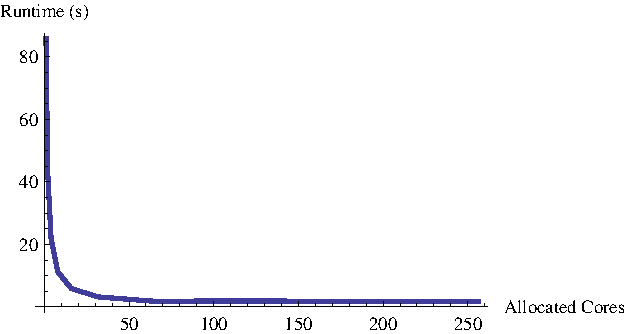
\includegraphics[width=84.5mm]{strongPlotOne.pdf}
    \caption{Runtime as core count increases on the 4890 with a fixed resolution ($400\times400$); smaller values are better}
    \label{fig:strongPlotOne}
\end{figure}

\begin{figure}
    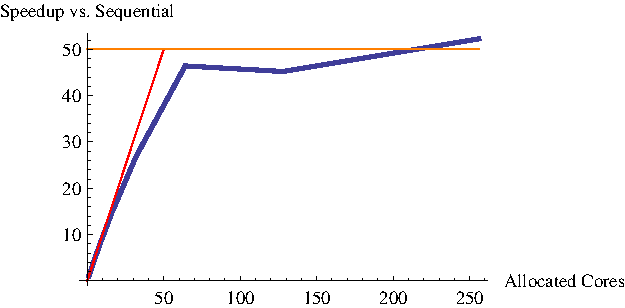
\includegraphics[width=84.5mm]{strongPlotTwo.pdf}
    \caption{Speedup as core count increases (measured against the single-core run) on the 4890 with a fixed resolution ($400\times400$); the orange line is the theoretical maximum speedup, given linear scaling and 50 execution units (800 cores / 16 cores per unit); the red line is a linear speedup curve; larger values are better}
    \label{fig:strongPlotTwo}
\end{figure}

One can see in figure \ref{fig:strongPlotTwo} that this implementation is strongly scalable; the speedup is almost perfectly linear as the core count increases. It should be noted that since the 4890 only has a maximum of 50 compute units, the linear increase is only maintained until we reach 50 cores; after that, the performance gains plateau as they should.

\subsection{Large- vs. Small-scale Parallelism}

\begin{figure}
    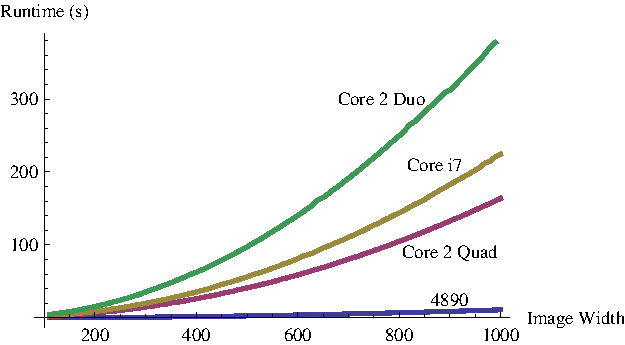
\includegraphics[width=84.5mm]{runtimePlot.pdf}
    \caption{Runtime vs. Resolution on all hardware; smaller values are better}
    \label{fig:runtimePlot}
\end{figure}

\begin{figure}
    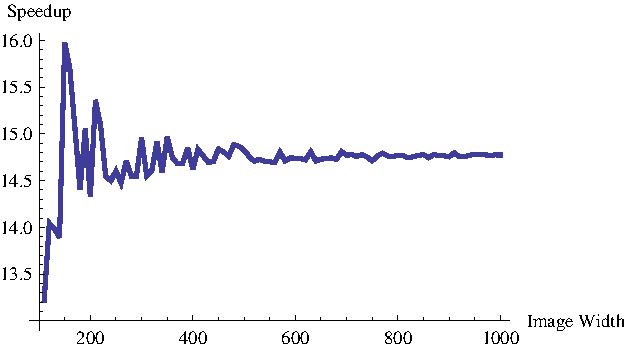
\includegraphics[width=84.5mm]{speedupPlot.pdf}
    \caption{Speedup of fastest GPU (4890) over fastest CPU (Core 2 Quad) as resolution increases; larger values are better}
    \label{fig:speedupPlot}
\end{figure}

As one can see in figure \ref{fig:runtimePlot}, the GPU significantly outperforms all of the CPUs. This is not surprising, as it can perform more than an order of magnitude more parallel computations, but it does validate the premise of this experiment.

Figure \ref{fig:speedupPlot} shows that our implementation converges to an approximately 14.7x speedup (between the fastest of each class of hardware, namely, the 4890 and Core 2 Quad) as the resolution of the output image increases. Noise in the speedup values with smaller images is likely due to measurement error and the overhead and unpredictability involved when copying data to/from video memory.

It should be noted that these speedup values are across different pieces of hardware at different core clock speeds, and, as such, do not represent the actual parallel speedup gained (for that, look at section \ref{strongScaling}). This is, instead, a representation of the performance potentially gained by moving computation to the GPU.

\subsection{Cost Effectiveness of Hardware}

\begin{figure}
    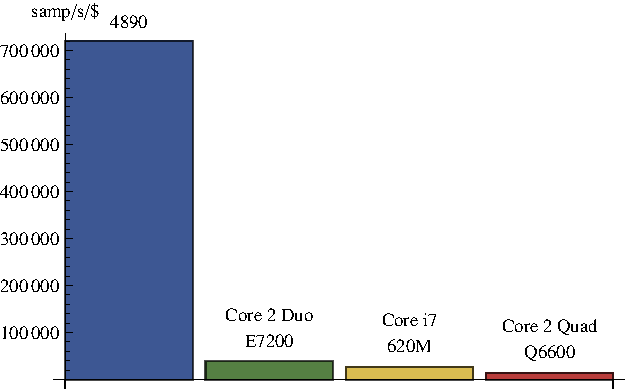
\includegraphics[width=84.5mm]{dollarPlot.pdf}
    \caption{Samples per second per dollar with a fixed resolution ($500\times500$); larger values are better}
    \label{fig:costEffectiveness}
\end{figure}

\begin{figure}
    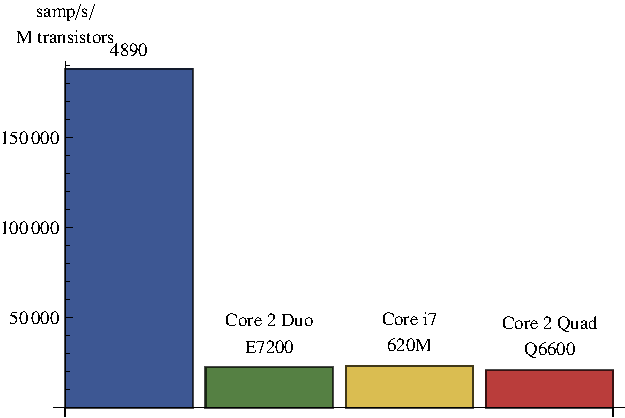
\includegraphics[width=84.5mm]{transistorPlot.pdf}
    \caption{Samples per second per million transistors with a fixed resolution ($500\times500$); larger values are better}
    \label{fig:transistorPlot}
\end{figure}

\begin{figure}
    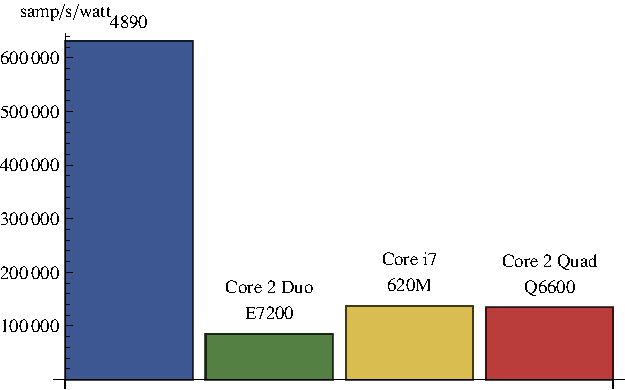
\includegraphics[width=84.5mm]{wattPlot.pdf}
    \caption{Samples per second per heavy-load watt with a fixed resolution ($500\times500$); larger values are better}
    \label{fig:wattPlot}
\end{figure}

One oft-cited measure of the performance of a computational device is its {\it performance-per-dollar}; this is especially of interest for consumers with budgets or people building large computation clusters. In order to measure performance-per-dollar, we have to define {\it performance} in the context of our problem. In all of the plots in this section, performance is measured as the number of samples per second. Figures \ref{fig:costEffectiveness}, \ref{fig:transistorPlot}, and \ref{fig:wattPlot} all use a 500$\times$500 image, with 2000 samples per pixel, for $500,000,000$ total samples.

Figure \ref{fig:costEffectiveness} illustrates the performance-per-dollar of our four devices. As is quite evident already, the 4890 --- though in the same price range as most of the other devices, and significantly cheaper than the Core 2 Quad --- manages to dominate the chart. It's safe to say that if an institution is looking into buying a large number of a particular device for scientific computation, they should seriously consider looking into high-end graphics cards. Indeed; each dollar spent on a 4890 goes 18 times farther, performance-wise, than it would if spent on the next-most-cost-effective chip, the Core 2 Duo E7200.

Another important point when considering the cost of various pieces of hardware is how much it will cost to run. One way to measure this is to consider the power efficiency of the chip, in terms of performance-per-watt. Again using the same measure of performance from our performance-per-dollar comparison, we can see in figure \ref{fig:wattPlot} that the GPU continues to dominate, even though it requires three times more energy to run than its closest competitor, the Core 2 Quad. As one might expect, the older --- thus, less power efficient --- Core 2 Duo falls behind the other CPUs on this scale: though it was the performance-per-dollar winner out of the three CPUs, it would cost significantly more than the other two to run for any period of time.

\section{Future Work}

There are quite a few things which have come up while developing this project that would be interesting to implement if we were to continue work on the codebase.

\subsection{Camera Transformation}

\label{cameraTransformation}

One key feature that is missing from the current implementation is the ability to manipulate the "camera" location, changing your viewport on the orbital cloud. Implementing this would add a bit of complexity, but would allow for interesting video rendering --- for example, video of the camera spinning around the atom, providing a better idea of the actual shape of the cloud. It can be hard --- without prior knowledge --- to comprehend the shape of the cloud from our current visualization.

In addition, if the number of samples was sufficiently reduced, or a fast enough video card was obtained, one could implement {\it live} manipulation of the camera's view, which could assist in inspection of the orbital cloud to an even greater extent.

\subsection{Slicing}

\begin{figure}
    
\includegraphics[width=84.5mm]{320-slice.png}
    \caption{A slice through the 3-2-0 orbital of the hydrogen atom}
    \label{fig:slice}
\end{figure}

Section \ref{cameraTransformation} covered the ideal solution to the problem of comprehending the shape of the orbital from our 2D representation --- however, if that solution proved to be too challenging, one could instead generate an animation of slices through the cloud, each slice being similar to figure \ref{fig:slice}

\subsection{Coloring}

\subsection{Generalization of Parameters}

\section{Conclusion}

\section{Code}

All of the code developed for this project is available under the two-clause BSD license, and is hosted on GitHub:

\url{http://github.com/hortont424/orbitals}

\url{git://github.com/hortont424/orbitals.git}

The code has only been tested with the Apple and ATI OpenCL compilers, but should work with few to no changes on NVIDIA's SDK.

\bibliographystyle{acmsiggraph}
\nocite{*}
\bibliography{paper}

\end{document}